\subsection{Introduction}

We test three related hypotheses:

\begin{enumerate}
\def\labelenumi{\arabic{enumi}.}
\item
  \emph{species co-occurance}: closely-related predators occur together
  more frequently than less-related predators, due to their similar
  habitat requirements. Additionally, very closely related species never
  co-occur because they are too similar.
\item
  \emph{diet similarity}: similarity in diet (as measured by feeding
  trials) decreases with phylogenetic distance.
\item
  \emph{ecosystem-level effects}: similarity in the effect of predators
  on whole ecosystems declines with phylogenetic distance. Additionally,
  the non-additive effect of predators will have a greater absolute
  value when their phylogenetic diversity is larger.
\end{enumerate}

\subsection{Methods}

\subsection{Results}

\subsubsection{metabolic capacity and phylogenetic distance}

\begin{verbatim}
## [1] "insects.to.leeches.csv"            
## [2] "odonata-Tabanidae.csv"             
## [3] "tabanidae_culidicae_ie_Diptera.csv"
\end{verbatim}

We identified 14 in the 2008 dataset as predators. These predators vary
in taxonomic relatedness: from congeners (\emph{Bezzia} sp.
(Diptera:Ceratopogonidae) with two species, \emph{Leptagrion} sp.
(Odonata:Coenagrionidae) with three) to confamilials (three species of
Tabanidae and two of Empididae, all Diptera). Three families of Diptera
are represented by a single species each: Dolichopodidae, Corethrellidae
and Chironomidae. The deepest taxonomic divide is between all insects
present and a species of leech (Annelida:Hirudinidae). Node age data was
available for all but the shallowest nodes of the tree, where either a
lack of taxonomic information (e.g.~Tabanidae) or a lack of phylogenetic
studies (e.g. \emph{Leptagrion}) prevented more information from being
included. These branches were left as polytomies, and were all assigned
identical, arbitrary and short branch lengths (15 Mya).

We obtained node age estimates for all 7 internal nodes of the tree.
These were usually provided by only a single study, with more studies
available for deeper nodes: Insecta--Hirudina (n=5, 543 to 700 Mya),
Odonata--Tabanidae (n=4, 151 to 543 Mya) and Tabanidae--Diptera (n=7,
151 to 543 Mya). We used the median estimate of age for these nodes.

In 2008, insects were counted and measured in an observational study of
25 bromeliads. Across all bromeliads, predator species differed widely
in metabolic capacity, from 0.0062 for a species of Empidid, to 0.4804
for the abundant predator \emph{Leptagrion andromache}. Predators often
co-occured in bromeliads ($3.52 \pm 3.1107$ per plant). However, the
euclidian distance between the total metabolic capacity of two predators
did not show any relationship with phylogenetic distance between them
(F\textsubscript{1,89}=1.5558,P=0.2155).

\subsubsection{diet similarity and phylogenetic distance}

All predators showed a very generalist diet breadth. However, more
phylogenetically distinct predators preferred slightly more distant
prey, as measured by euclidian distance between feeding trial outcomes
(F\textsubscript{1,19}=5.1641,P=0.0349) Regression was weighted by the
number of trials conducted.

\subsubsection{Ecosystem-level effects and phylogenetic distance}

All increases in predator phylogenetic diversity beyond damselflies
resulted in a reduction of prey mortality.

predator addition treatments did not differ strongly from predator-free
controls. We did not find significant differences for FPOM,
decompositon, or bromeliad growth. However, we did find results for N15
uptake into bromeliads. Our strongest differences were in insect
survivorship, which decreased in all predator treatments relative to
control.

\subsubsection{Figures}

\begin{figure}[htbp]
\centering
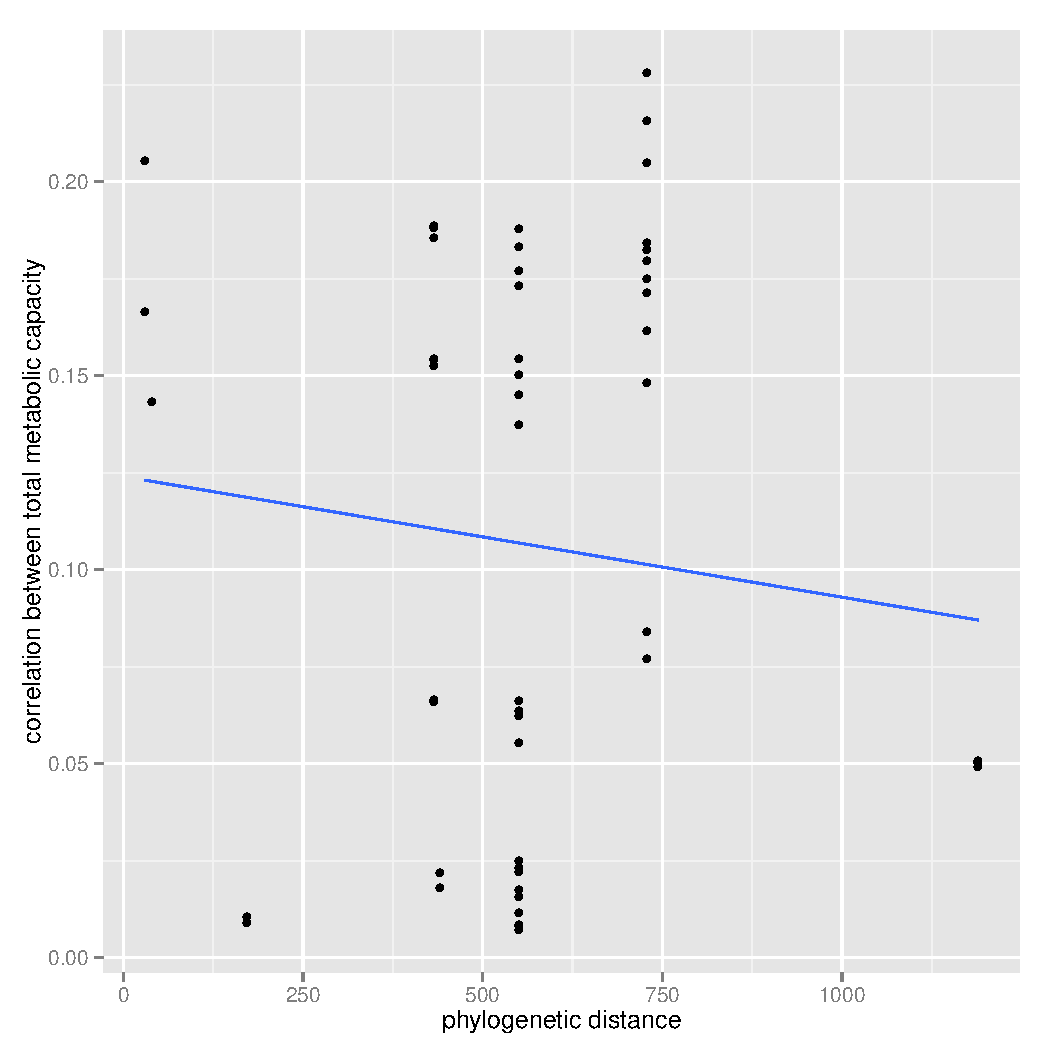
\includegraphics{figure/FIG_metabolic_occurance_as_phylo.pdf}
\caption{FALSE}
\end{figure}

\begin{figure}[htbp]
\centering
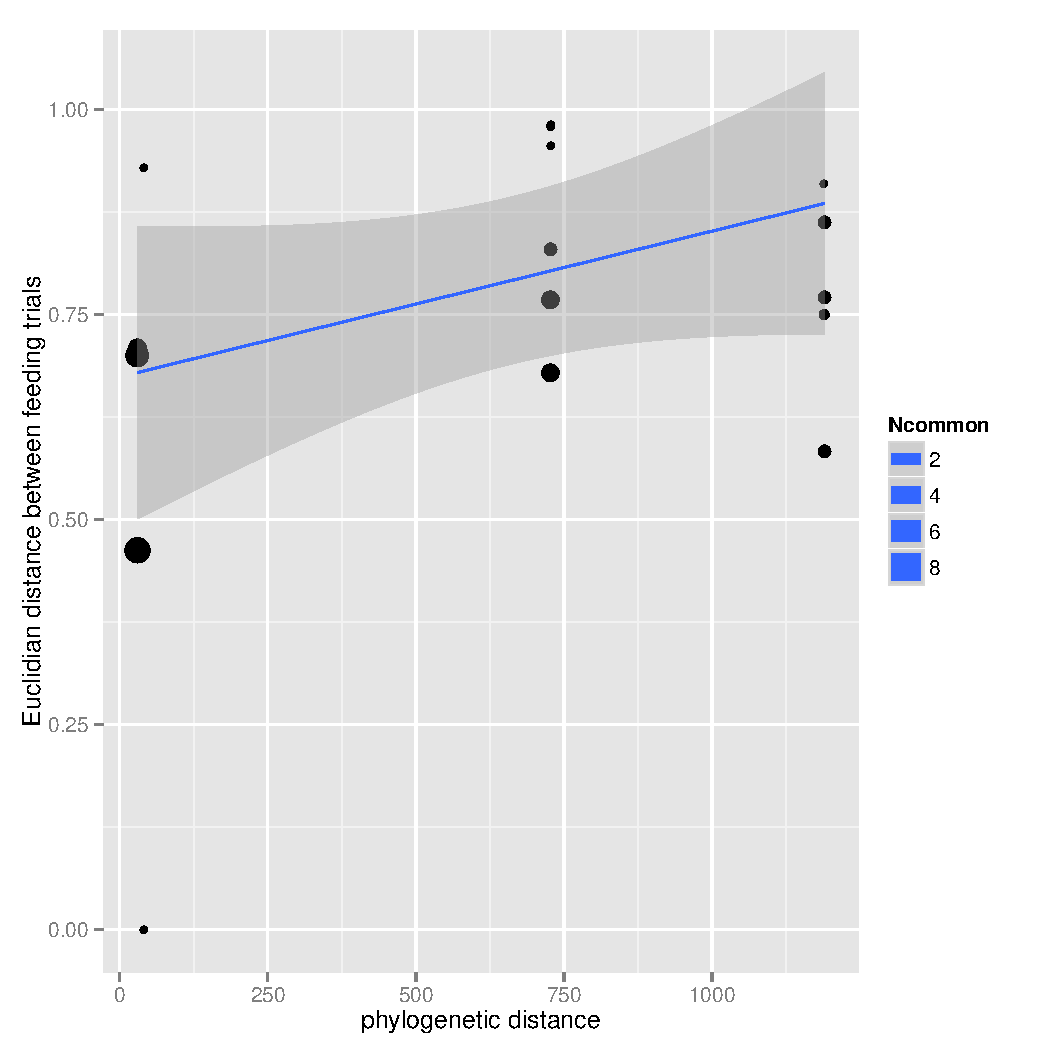
\includegraphics{figure/FIG_feeding_trial_as_phylo.pdf}
\caption{FALSE}
\end{figure}

\begin{figure}[htbp]
\centering
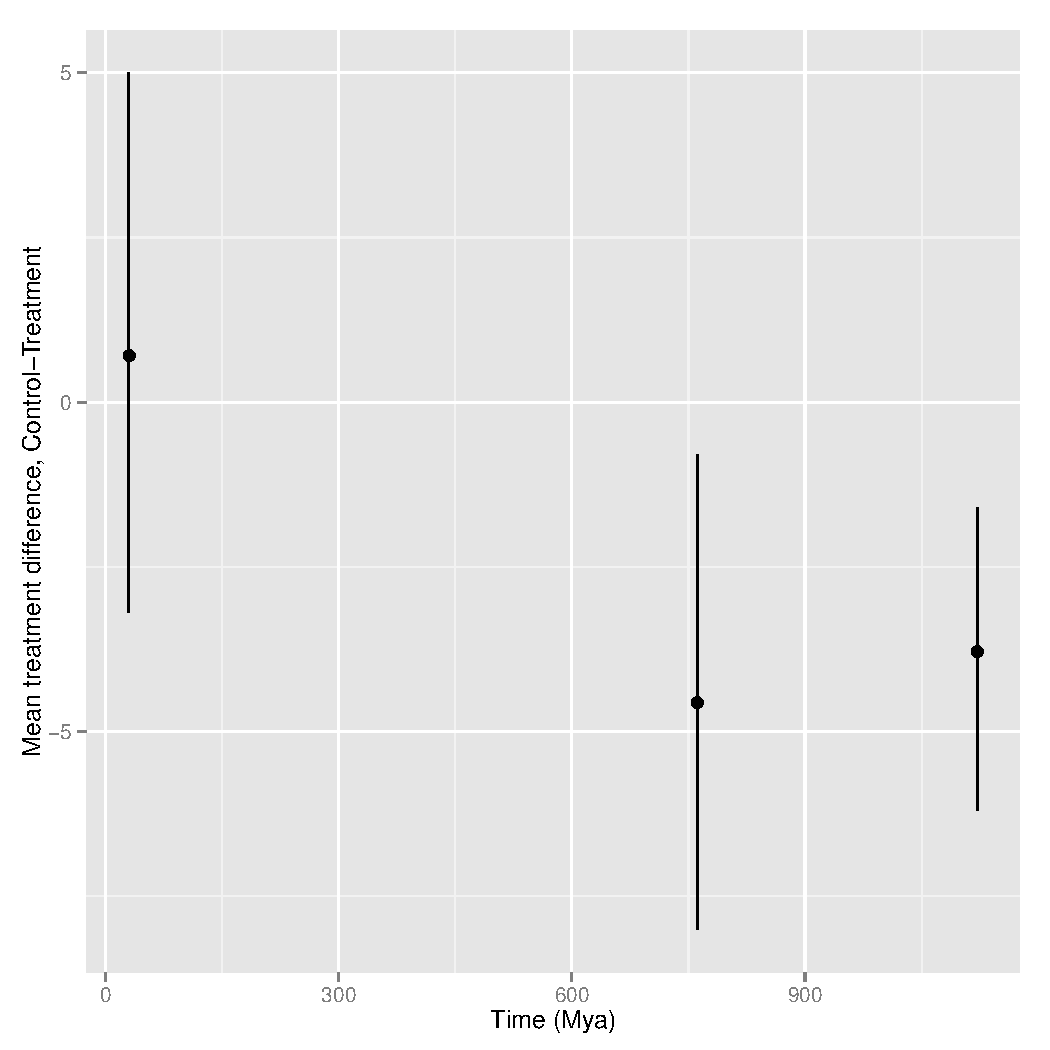
\includegraphics{figure/FIG_PD_experiment_nonadditive.pdf}
\caption{FALSE}
\end{figure}

\begin{figure}[htbp]
\centering
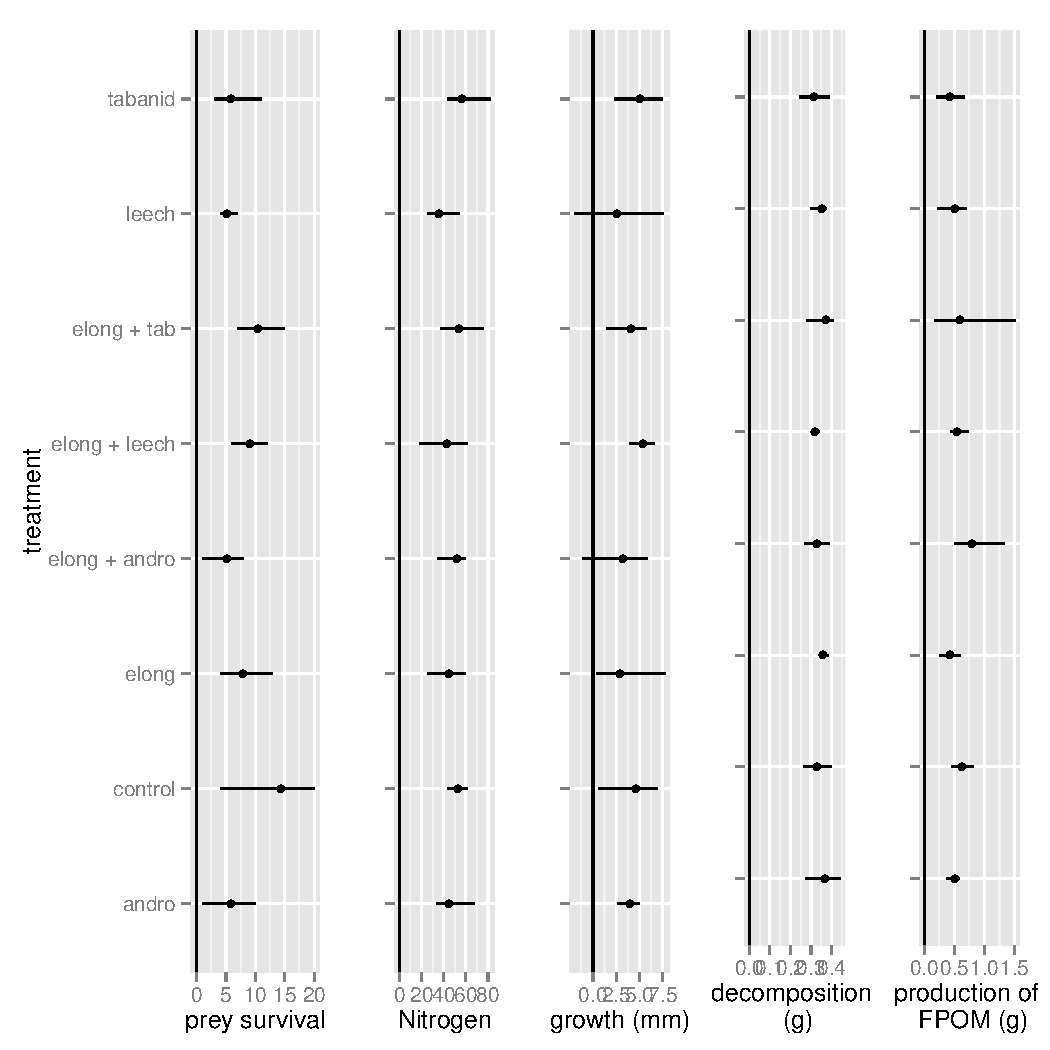
\includegraphics{figure/FIG_experiment_responses.pdf}
\caption{FALSE}
\end{figure}

controls not really differen

\subsection{Discussion}

\subsection{Works Cited}
